\documentclass[slovene,11pt,a4paper]{article}
\usepackage[margin=1.7cm,bottom=3cm,foot=1.5cm]{geometry}
\setlength{\parindent}{0pt}
\setlength{\parskip}{0.5ex}

\usepackage[pdftex]{graphicx}
\usepackage{pgffor}

% \usepackage{a4wide} %najaci package
\usepackage[utf8]{inputenc}
\usepackage[slovene]{babel}
\usepackage{color}
\usepackage{graphicx}
\usepackage{subfigure}
\usepackage{imakeidx}
\usepackage{adjustbox}
\usepackage{float}
\usepackage{amsmath}
\usepackage{mathtools}
\usepackage{tikz}
\usepackage{amssymb}
\usepackage{listings}
\usepackage{siunitx}
\usepackage{hyperref}
\usepackage{amsfonts}
\usepackage{mathrsfs}


%\def\phi{\varphi}
\def\eps{\varepsilon}
\def\theta{\vartheta}

\newcommand{\thisyear}{2024/25}

\renewcommand{\Re}{\mathop{\rm Re}\nolimits}
\renewcommand{\Im}{\mathop{\rm Im}\nolimits}
\newcommand{\Tr}{\mathop{\rm Tr}\nolimits}
\newcommand{\diag}{\mathop{\rm diag}\nolimits}
\newcommand{\dd}{\,\mathrm{d}}
\newcommand{\ddd}{\mathrm{d}}
\newcommand{\ii}{\mathrm{i}}
\newcommand{\lag}{\mathcal{L}\!}
\newcommand{\ham}{\mathcal{H}\!}
\newcommand{\four}[1]{\mathcal{F}\!\left(#1\right)}
\newcommand{\bigO}[1]{\mathcal{O}\!\left(#1\right)}
\newcommand{\sh}{\mathop{\rm sinh}\nolimits}
\newcommand{\ch}{\mathop{\rm cosh}\nolimits}
\renewcommand{\th}{\mathop{\rm tanh}\nolimits}
\newcommand{\erf}{\mathop{\rm erf}\nolimits}
\newcommand{\erfc}{\mathop{\rm erfc}\nolimits}
\newcommand{\sinc}{\mathop{\rm sinc}\nolimits}
\newcommand{\rect}{\mathop{\rm rect}\nolimits}
\newcommand{\ee}[1]{\cdot 10^{#1}}
\newcommand{\inv}[1]{\left(#1\right)^{-1}}
\newcommand{\invf}[1]{\frac{1}{#1}}
\newcommand{\sqr}[1]{\left(#1\right)^2}
\newcommand{\half}{\frac{1}{2}}
\newcommand{\thalf}{\tfrac{1}{2}}
\newcommand{\pd}{\partial}
\newcommand{\Dd}[3][{}]{\frac{\ddd^{#1} #2}{\ddd #3^{#1}}}
\newcommand{\Pd}[3][{}]{\frac{\pd^{#1} #2}{\pd #3^{#1}}}
\newcommand{\avg}[1]{\left\langle#1\right\rangle}
\newcommand{\norm}[1]{\left\Vert #1 \right\Vert}
\newcommand{\braket}[2]{\left\langle #1 \vert#2 \right\rangle}
\newcommand{\obraket}[3]{\left\langle #1 \vert #2 \vert #3 \right \rangle}
\newcommand{\hex}[1]{\texttt{0x#1}}

\renewcommand{\iint}{\mathop{\int\mkern-13mu\int}}
\renewcommand{\iiint}{\mathop{\int\mkern-13mu\int\mkern-13mu\int}}
\newcommand{\oiint}{\mathop{{\int\mkern-15mu\int}\mkern-21mu\raisebox{0.3ex}{$\bigcirc$}}}

\newcommand{\wunderbrace}[2]{\vphantom{#1}\smash{\underbrace{#1}_{#2}}}

\renewcommand{\vec}[1]{\overset{\smash{\hbox{\raise -0.42ex\hbox{$\scriptscriptstyle\rightharpoonup$}}}}{#1}}
\newcommand{\bec}[1]{\mathbf{#1}}


\title{
\sc\large Matematično-fizikalni praktikum \thisyear\\
\bigskip
\bf\Large 5.~naloga: Hitra Fourierova transformacija in korelacijske funkcije
}
\author{Tadej Tomažič}
\date{}

\makeindex[columns=3, title=Alphabetical Index, intoc]

\begin{document}


\pagenumbering{gobble} 
\author{Tadej Tomažič}
\date{\today}

\maketitle

\newpage
\pagenumbering{arabic}
\tableofcontents
\listoffigures
\newpage
\section{Navodila}

Diskretno Fourierovo transformacijo smo definirali kot
\begin{equation*}
H_k = \sum_{n=0}^{N-1}
h_n \exp(2 \pi \ii k n / N),
\qquad k=-\tfrac{N}{2},\dots ,\tfrac{N}{2},
\end{equation*}
oziroma
\begin{equation*}
H_k = \sum_{n=0}^{N-1} W_N^{nk} h_n,
\qquad W_N = \exp(2 \pi \ii / N).
\end{equation*}
Ta postopek ima očitno časovno zahtevnost $N^2$. Račun pa je
mogoče izvesti tudi z bistveno manj operacijami. Osnovni premislek
je razcep
\begin{equation*}
H_k = H_{k}^\mathrm{sod} + W_N^k H_{k}^\mathrm{lih} \>,  
\end{equation*}
kjer smo transformiranko $H$ izrazili s transformacijama njenih
sodih in lihih členov, pri čemer je vsota vsake od transformacij zdaj dolžine N/2.
 Gornjo relacijo lahko uporabljamo rekurzivno:
če je $N$ enak potenci števila 2, lahko rekurzijo razdrobimo
do nizov, ki imajo samo še en člen. Zanj je transformacija
identiteta. Za obrat pri eni vrednosti frekvence (pri danem $m$)
je potrebno na vsakem koraku rekurzije le eno množenje s potenco
$W$, korakov pa je $\log_2 N$.  Skupna časovna zahtevnost je torej
le še $N\log_2 N$.

Da ne iščemo pripadnikov niza po vsej tabeli, si podatke
preuredimo. Lahko je pokazati, da je v prvotni tabeli treba med
seboj zamenjati podatke, katerih vrstna števila v binarnem zapisu
so obrnjena: v novem redu jemljemo člene kar po vrsti. Tudi
potenc $W$ ne izražamo vedno znova s sinusi in kosinusi,
pač pa jih računamo z rekurzijo.  Tak ali podoben postopek
je osnova vseh algoritmov hitre Fourierove transformacije (FFT).

Z neko transformacijo iz družine FFT bomo izračunali korelacijsko
funkcijo dveh signalov. Korelacija periodičnih funk\-cij $g(t)$ in $h(t)$
s periodo $T$ je definirana kot:
\begin{equation*}
\phi_{gh}(\tau)=\frac{1}{T}\int\limits_0^{T} g(t+\tau)\,h(t)\dd t \>,  
\end{equation*}
oziroma diskretno
\begin{equation*}
  \phi_{gh}(n)= \frac{1}{N}\sum_{k=0}^{N-1} g_{k+n}\, h_k \>.
\end{equation*}
Računamo torej skalarni produkt funkcij, ki sta časovno premaknjeni
za $\tau$ oziroma $n$. Če je za določeno vrednost premika ta
funkcija višja kot v okolici, potem to pomeni, da sta si funkciji
podobni, le da ju je treba premakniti, da se to vidi.

V primeru, da sta funkciji (signala), ki ju primerjamo, enaki,
računamo njuno {\sl avtokorelacijsko funkcijo\/}: ta je mera
za to, ali signal ostaja s pretekanjem časa sam sebi podoben.
Če je signal slabo koreliran (sam s sabo), korelacija $\phi_{hh}(n)$
relaksira h kvadratu povprečnega signala $\langle h\rangle^2$, kjer je
\begin{equation*}
\langle h\rangle = \frac{1}{N} \sum_{k=0}^{N-1} h_k \>.  
\end{equation*}
Iz lokalnih maksimov v avtokorelacijski funkciji sklepamo
na periodičnosti, bodisi popolne ali približne.
Pri periodičnih signalih je tudi avtokorelacijska funkcija
striktno periodična, za stohastične procese pa je značilna
eksponentna avtokorelacijska funkcija.
še bolj nas zanima, kako {\sl hitro\/} se korelacija izgublja:
računamo rajši reskalirano obliko avtokorelacije
\begin{equation*}
\widetilde{\phi}_{hh}(n) = 
{ \phi_{hh}(n) - \langle h\rangle^2 \over \phi_{hh}(0) - \langle h\rangle^2 } \>,  
\end{equation*}
kjer je imenovalec nekakšno merilo za  varianco signala,
\begin{equation*}
\sigma^2 = \phi_{hh}(0) - \langle h\rangle^2 
= \frac{1}{N} \sum_{k=0}^{N-1} \left( h_k - \langle h\rangle \right)^2 \>.  
\end{equation*}
Pri zgornjih enačbah moramo še ``peš'' poskrbeti za periodično
zaključenost signala pri $n=N$, torej da je perioda enaka velikosti
vzorca.  Če tega ne moremo narediti, je bolj pravilna definicija
avtokorelacije
\begin{equation*}
\phi_{hh}(n)= \frac{1}{N-n}\sum_{k=0}^{N-n-1} h_{k+n}\, h_k \>.  
\end{equation*}
Praktičen račun po zgornji formuli lahko postane za velike
vzorce prezamuden.  Avtokorelacijo rajši računamo s FFT (DFT) $\mathcal{F}$,
saj je korelacija obratna Fourierova transformacija ${\cal F}^{-1}$
produkta Fourierovih transformacij ${\cal F}$, torej z $G={\cal F}g$ in $H={\cal F}h$ dobimo
\begin{equation*}
\phi_{gh}(n) = \frac{1}{N-n}\mathcal{F}^{-1} \left[ G \cdot (H)^\ast \right]
\end{equation*}
oziroma
\begin{equation*}
  \phi_{hh}(n) = \frac{1}{N-n}{\cal F}^{-1} \left[ \, | H |^2 \, \right] \>.
\end{equation*}
Za račun s FTT signale dolžine $N$ najprej prepišemo v dvakrat
daljše, periodično zaključene podatkovne nize, $\widetilde{h}_n = h_n$,
$\widetilde{h}_{n+N} = 0$ za $n = 0, \ldots, N-1$
in $\widetilde{h}_{n+2N} = \widetilde{h}_{n}$.
Tedaj se avtokorelacija zapiše v obliki
\begin{equation*}
\phi_{hh}(n)={1\over N-n}\sum_{k=0}^{2N-1}\widetilde{h}_{k+n}\,\widetilde{h}_k \>,  
\end{equation*}
kar lahko izračunamo s FFT.

\bigskip

{\it Naloga\/}: Na spletni strani MF praktikuma najdeš posnetke
oglašanja velike uharice, naše največje sove.  Posneti sta
dve sovi z minimalnim ozadjem ({\tt bubomono} in {\tt bubo2mono})
in nekaj mešanih signalov, ki zakrivajo njuno oglašanje
({\tt mix}, {\tt mix1}, {\tt mix2} in {\tt mix22}).
V signalih {\tt mix2} in {\tt mix22} je oglašanje sove
komaj še zaznavno.  Izračunaj avtokorelacijsko funkcijo 
vseh signalov in poskusi ugotoviti, za katero sovo gre
pri teh najbolj zašumljenih signalih!

Poglejte si rutine {\tt four1\/} iz Numerical Recipes
ali knjižnice {\tt fftw3}, ki je še dosti hitrejša. V okolju Python
so te rutine vključene v 'fft' paket. 
(Pri tako velikih vzorcih je skorajda nujno uporabiti FFT
namesto počasne navadne DFT.)

\bigskip

{\it Dodatna naloga\/}: Izračunaj še avtokorelacijsko funkcijo
za kak signal, ki ga posnameš sam ali za kak proces, za katerega
sam poiščeš ustrezne podatke.

\section{Rešitev}

Najprej si poglejmo avtokorelacijo za obe sovi.
\begin{figure}[h]
    \centering
    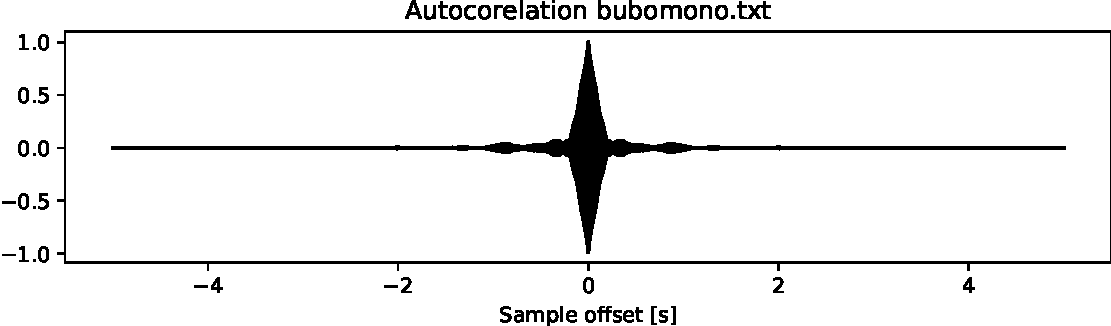
\includegraphics[width=12cm]{pdfs/bubomono.txt_acor.pdf}
    \vspace{10pt}
    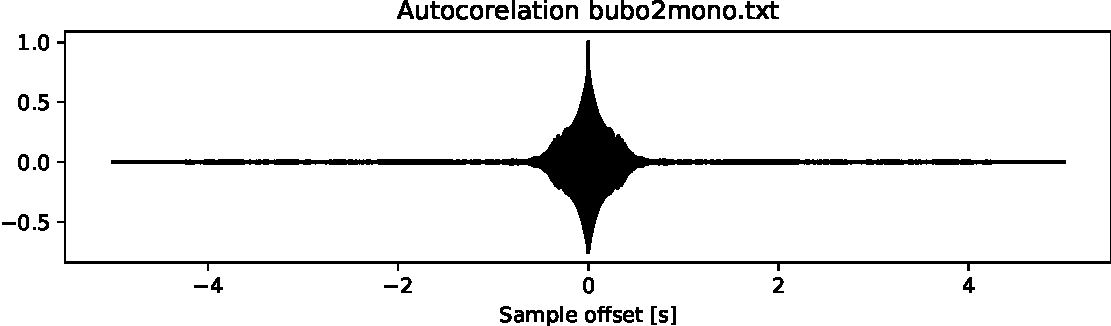
\includegraphics[width=12cm]{pdfs/bubo2mono.txt_acor.pdf}
    \caption{Avtokorelacija signala sov}
\end{figure}

Preden sem koreliral signal sem vektorja samplov normiral, tako da je
"najmočnejši" signal 1. To pomeni \[\|x\|_\infty = \max_i |x_i|\]

Poglejmo si še korelacije med sovami in posnetki:
\newpage
\begin{figure}[h]
    \centering
    \foreach \mix in {mix, mix1, mix2, mix22} {
        \foreach \sova in {bubomono, bubo2mono}{
            \includegraphics[width=8cm]{pdfs/cor_\mix.txt_\sova.txt.pdf}
        }
    }
    \caption{Korelacija sov in posnetkov iz narave}
\end{figure}
Tukaj je bila normalizacija drugače izbrana. Tukaj je bila narejena normalizacija korelacije. Če je varianca signala a $\sigma_a$,
potem je $ \mathbf{x} = \mathbf{x} / \left(\sigma_a \sigma_b |\mathbf{b}|\right)$. Sigma je izračunana z \verb|numpy.std()|.


Hitrosti so precej dolgčasno pričakovane ampak vseeno.
\begin{figure}[h]
    \centering
    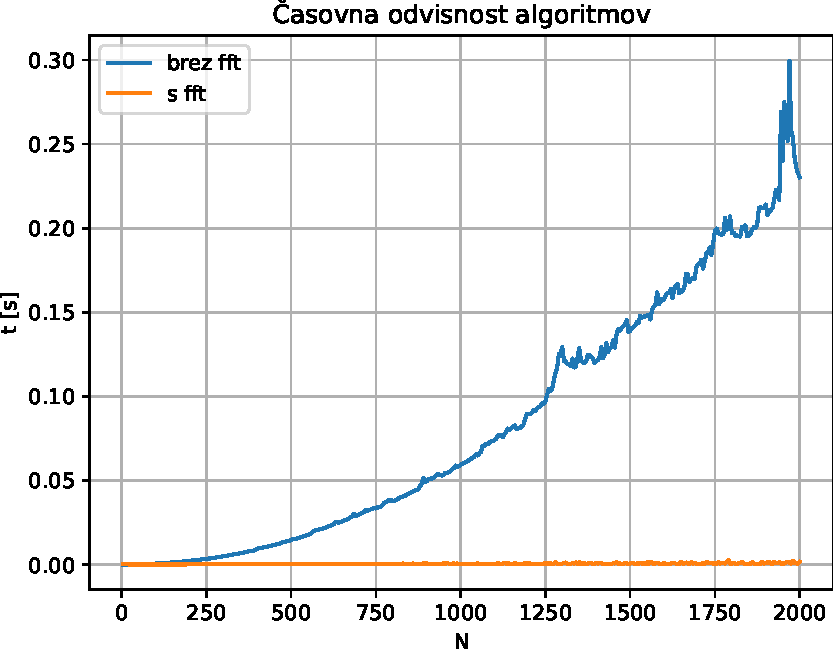
\includegraphics[width=8cm]{pdfs/cas-lin.pdf}
    \vspace{10pt}
    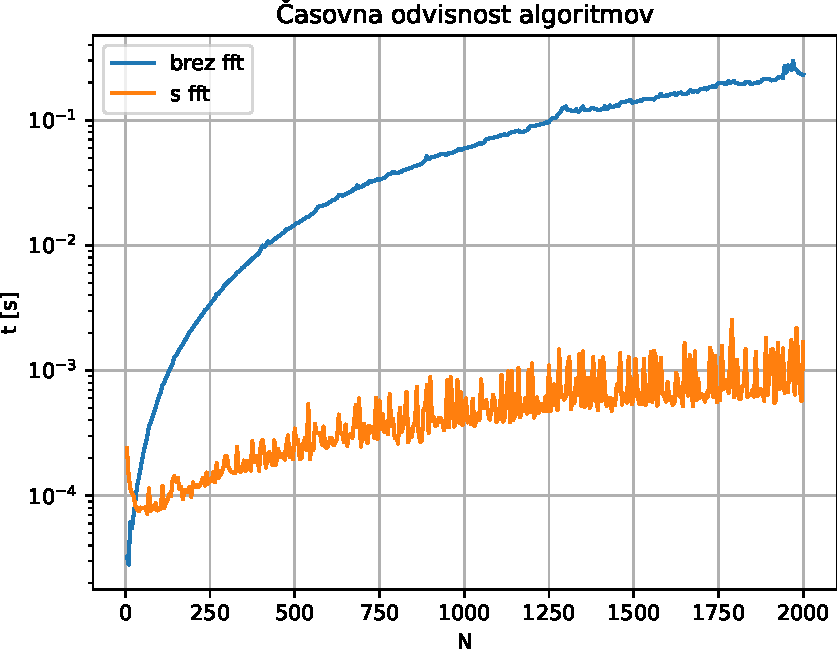
\includegraphics[width=8cm]{pdfs/cas-log.pdf}
    \caption{Hitrost algoritmov}
\end{figure}
\newpage
\section{Dodatna naloga}
Posnel sem dva človeka m in ž ko izgovarjata aaaaaaaaaaaa. Posnel sem jih tudi
ko bereta slovar. Gledal sem ali lahko spet zaznam ali gre za ž glas ali m glas.
Poglejmo si spektra njunega glasu.
\begin{figure}[h]
    \begin{center}
        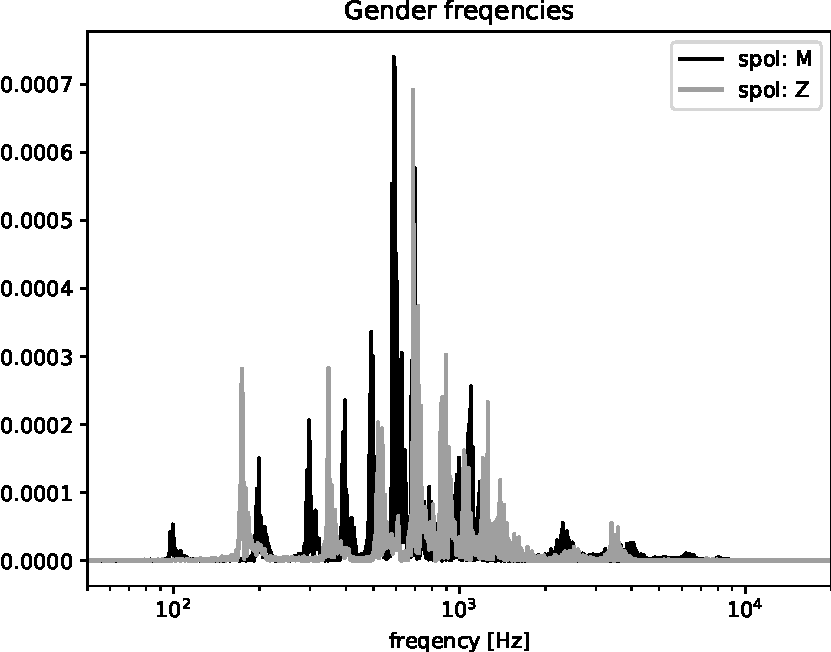
\includegraphics[width=12cm]{pdfs/fft_spol.pdf}
    \end{center}
    \caption{Barva glasu moškega in ženske}
\end{figure}

% Glasova sta bila prej normirana, saj je bil moški glas posnet bližje mikrofona.
% Poglejmo si zopet korelacijo med posnetki:
% \foreach \gender in {Z, M} {
%     \foreach \mix in {Glas\ 001, Glas\ 002}{
%         pdfs/cor_\gender_\mix.pdf 
%     }
% }
\begin{figure}[h]
    \begin{center}
        
    \foreach \gender in {Z, M} {%
        \foreach \mix in {001, 002} {%
            \includegraphics[width=8cm]{pdfs/cor_\gender_Glas\space\mix.pdf}%    
        }%
        \par
}%
    \end{center}
    
    \caption{Korelacija glasa človeka in posnetkov iz branja slovarja}
\end{figure}
\end{document}
